\documentclass[12pt,a4paper]{report}
\usepackage{geometry}
\usepackage{slashbox}
\geometry{
	a4paper,
	total={170mm,257mm},
	left=20mm,
	top=20mm,
}
\usepackage{graphicx}
\usepackage{pdfpages}

\usepackage{polski}
\usepackage[utf8]{inputenc}

\begin{document}
	
	\begin{titlepage}
		\newgeometry{top=5.5cm, bottom=3cm}
		
		\centering
		{\huge\bfseries Logika układów cyfrowych lab.\par}
		
		\vspace{0.5cm}
		Prowadzący: Antoni Sterna (E02-38m, wtorek 17:05) \\
	
		\vspace{1.1cm}
		{\Large sprawozdanie 1 - 2017.10.10\par}
		\vfill
		
		{\large\bfseries Jakub Dorda 235013\par}
		{\large\bfseries Marcin Kotas 235098\par}
		
		\vspace{1cm}
		\today \\ \LaTeX
		
		\restoregeometry
	\end{titlepage}
	
	%wprowadzenie
	
	{\large\bfseries 1. Wprowadzenie/cel ćwiczeń\\}
	
	Celem zadania było przećwiczenie metody Karnough na przykładzie tablicy prawdy podanej przez prowadzącego. Następnie należało przeprowadzić dwie minimalizację korzystając jedynie z bramek NAND lub NOR dla każdej minimalizacji. Z uzyskanych finalnie wzorów stworzono schematy ideowe układów logicznych. Poprawność przeprowadzonych obliczeń należało zweryfikować w praktyce z wykorzystaniem zestawu do prototypowania prostych układów logicznych. 
	
	%tabela prawdy&Karnaugh
	\vspace{0.8cm}
	{\large\bfseries 2. Tabele i minimalizacje}
	
	\begin{table}[h]
		\begin{minipage}{.5\textwidth}
			\caption{Tabela Prawdy}
			\vspace{0.4cm}
			\centering
			\begin{tabular}{cccc|l}
				a&b&c&d&y\\\hline
				0&0&0&0&0\\
				0&0&0&1&0\\
				0&0&1&0&0\\
				0&0&1&1&0\\\hline
				0&1&0&0&1\\
				0&1&0&1&1\\
				0&1&1&0&1\\
				0&1&1&1&1\\\hline
				1&0&0&0&1\\
				1&0&0&1&1\\
				1&0&1&0&1\\
				1&0&1&1&1\\\hline
				1&1&0&0&1\\
				1&1&0&1&1\\
				1&1&1&0&0\\
				1&1&1&1&0\\
			\end{tabular}
		\end{minipage}%
		\begin{minipage}{.5\textwidth}
			\caption{Tablica Karnaugh}
			\vspace{0.4cm}
			\centering
			\begin{tabular}{c|c|c|c|c}
				\backslashbox{ab}{cd}&00&01&11&10\\\hline
				       00&0 &0 & 0&0\\\hline
					   01&1 &1 & 1&1\\\hline
					   11&1 &1 & 0&0\\\hline
					   10&1 &1 & 1&1\\
			\end{tabular}
		\end{minipage} 
	\end{table}

	
	%minimalizacja
	
	{\bfseries Minimalizacja dla bramek NAND:}
	\begin{displaymath}
	y=\bar{a}b+a\bar{b}+b\bar{c}
	=b\cdot(\bar{a}+\bar{c})+a\cdot\bar{b}
	=\overline{\overline{b\cdot(\bar{a}+\bar{c})+a\cdot\bar{b}}}
	=\overline{\overline{b\cdot(\bar{a}+\bar{c})}\cdot\overline{a\cdot\bar{b}}}
	=\overline{\overline{b\cdot\overline{\overline{\bar{a}+\bar{c}}}}\cdot\overline{a\cdot\bar{b}}}
	=\overline{\overline{b\cdot\overline{a\cdot c}}\cdot\overline{a\cdot\bar{b}}}
	\end{displaymath}
	
	{\bfseries Minimalizacja dla bramek NOR:}
	\begin{displaymath}
	y=\bar{a}b+a\bar{b}+b\bar{c}
	=b\cdot(\bar{a}+\bar{c})+a\cdot\bar{b}
	=\overline{\overline{b\cdot(\bar{a}+\bar{c})}}+\overline{\overline{a\cdot\bar{b}}}
	=\overline{\overline{\overline{\bar{b}+\overline{(\bar{a}+\bar{c})}}+\overline{\bar{a}+b}}}
	\end{displaymath}
	
	%wzory
	
	{\bfseries Użyte wzory:}
	\begin{equation}
	\overline{a\cdot b}=\bar{a}+\bar{b}
	\end{equation}
	\pagebreak
	\begin{equation}
	\overline{a+b}=\bar{a}\cdot\bar{b}
	\end{equation}
	\begin{equation}
	\bar{\bar{a}}=a
	\end{equation}
	
	%schemat ideowy układu
	\vspace{0.5cm}
	{\large\bfseries 3. Schematy}
	
	\vspace{0.5cm}
	\begin{center}
		\makebox[\textwidth]{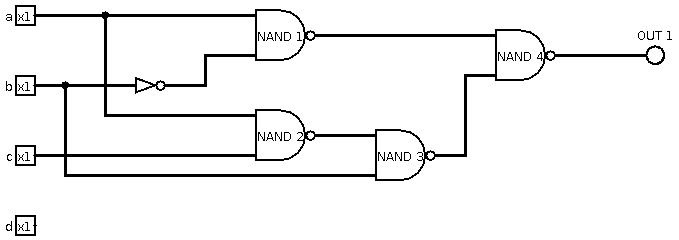
\includegraphics[width=\paperwidth - 40mm]{schem/circuit.png}}
		Schemat 1. Układ na bramkach NAND
	\end{center}
	
	\vspace{1.0cm}
	\begin{center}
		\makebox[\textwidth]{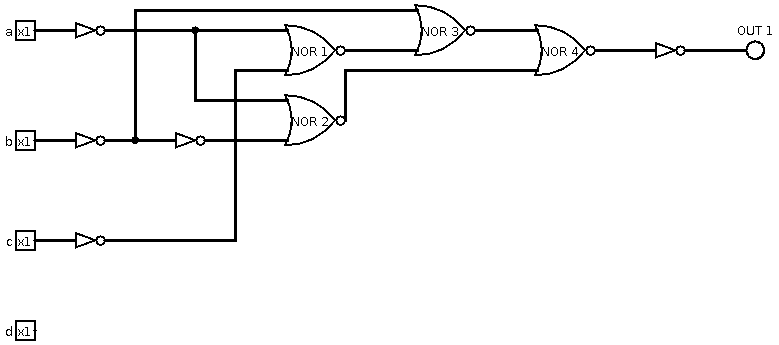
\includegraphics[width=\paperwidth - 40mm]{schem/circuit2.png}}
		Schemat 2. Układ na bramkach NOR
	\end{center}
	Wszystkie wejścia poprowadzone przez bramki NOR lub sygnał z wyjść 0 przełączników.\\ 
	
	%wnioski
	
	\vspace{0.5cm}
	{\large\bfseries 4. Wnioski/podsumowanie\\}
	
	Podczas przeprowadzania praktycznej części ćwiczenia najważniejszą kwestią okazało się systematyczne zrealizowanie uprzednio stworzonego schematu, organizacja pracy oraz umiejętność debugowania układu. W celu sprawdzenie poprawności działania należało przeprowadzić testy dla wszystkich możliwych kombinacji wejść w tym przypadku $2^3 = 8$ (3 wejścia ponieważ stan d nie ma znaczenia dla końcowego wyniku)
	
\end{document}